\documentclass[../kl11.tex]{subfiles}
\graphicspath{{\subfix{../images/}}}

\begin{document}
\section{Organische Chemie mit Aux-sicht}

Enantioselektive Synthesen spielen in der organischen Chemie eine große Rolle, beispielsweise um von Wirkstoffen nur das aktive Enantiomer zu erhalten. Eine sehr vielseitige Methode ist die \textsc{Evans}-Auxiliar-Chemie. Nachfolgend ist die Synthese des \textsc{Evans}-Auxiliars \textbf{3} dargestellt, ausgehend von einem in der Natur reichlich enantiomerenrein vorkommenden Stoff \textbf{1}. 

\begin{figure}[H]
    \centering
    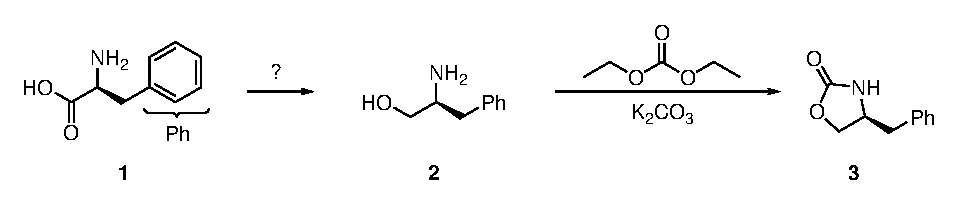
\includegraphics[width=0.9\textwidth]{2024/Abbildungen/Auxiliarchemie/1.eps}
\end{figure}

\renewcommand{\arraystretch}{1.2}

\enumaufgabe{\operator{Nenne} die biochemische Stoffklasse, der \textbf{1} angehört.}
\solution{Aminosäure, 1 P.}{2cm}
\enumaufgabe{\operator{Kreuze an}, welche der folgenden Reagenzienkombinationen für die Umsetzung von \textbf{1} zu \textbf{2} geeignet ist.}
\begin{tabularx}{\textwidth}{|X|C{1.5cm}|}\hline
    \ce{(H3C)2SO}, \ce{(COCl)2}, dann \ce{N(CH2CH3)3} & \emptybox \\\hline
    \ce{H2O}, \ce{HCl}	& \emptybox \\\hline
    \ce{MeOH}, \ce{BaCl2}	& \emptybox \\\hline
    \ce{S(CH3)2}, \ce{BH3}, \ce{BF3}  & \solutiontext{\checkedbox}{\emptybox} \\\hline
\end{tabularx}
\solutiontext{1 P. für richtiges Kreuz; falls ein Kreuz falsch: 0 P.}{} 
\\ 
Das \textsc{Evans}-Auxiliar \textbf{3} ist nur ein Hilfsstoff. Umgesetzt werden soll ein Säurederivat \textbf{4}, an welches vor der beabsichtigten Reaktion das \textsc{Evans}-Auxiliar \textbf{3} kovalent gebunden wird. 
\begin{figure}[H]
    \centering
    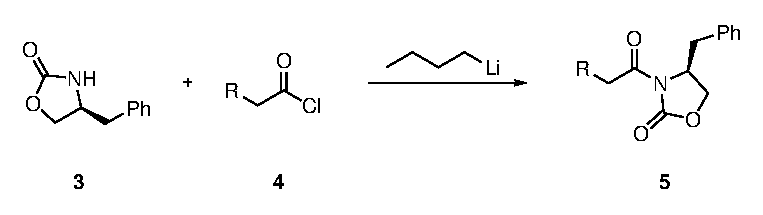
\includegraphics[width=0.8\textwidth]{2024/Abbildungen/Auxiliarchemie/2.eps}
\end{figure}

\enumaufgabe{\operator{Formuliere} den Reaktionsmechanismus der Bildung von \textbf{5}.\\ Hinweis: Das Reagenz n-BuLi darf vereinfachend als \ce{Li+Base-} geschrieben werden.}
\begin{framed}
\vspace{4cm}
\end{framed}
\solution{
Erste beiden Schritte je 1,5 P., letzter Schritt 1 P.; insg. 4 P.
\begin{figure}[H]
    \centering
    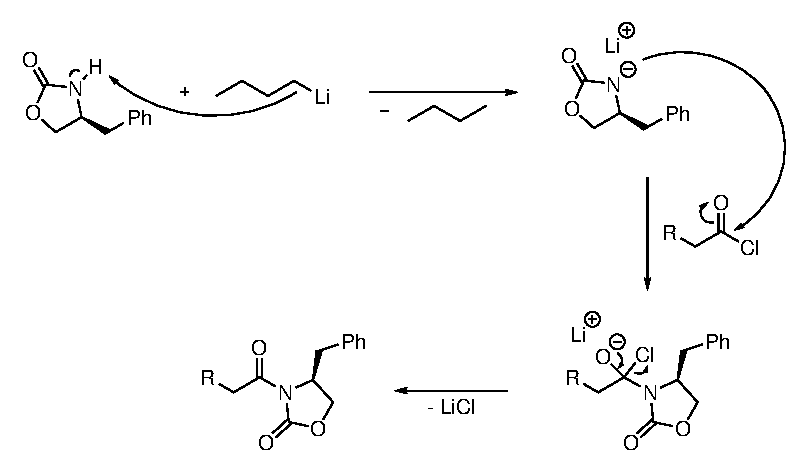
\includegraphics[width=0.8\textwidth]{2024/Abbildungen/Auxiliarchemie/L_c.eps}
\end{figure}}
{9cm}

Anschließend wird \textbf{5} enolisiert, wofür verschiedene Basen verwendet werden können. 

\begin{figure}[H]
    \centering
    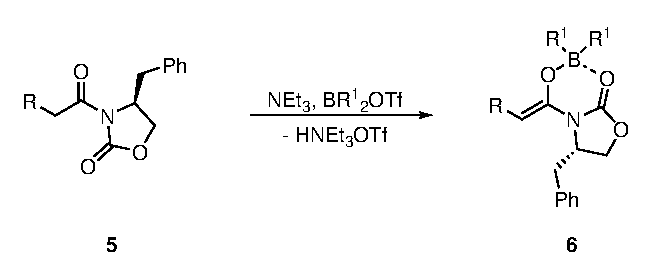
\includegraphics[width=0.68\textwidth]{2024/Abbildungen/Auxiliarchemie/3.eps}
\end{figure}

In diesem Beispiel wird das selektiv erhaltene (Z)-Enolat \textbf{6} durch Bor stabilisiert. Da Bor maximal vier Bindungen ausbilden kann, kann es neben den drei kovalenten Bindungen für genau eine koordinative Bindung als \textsc{Lewis}-Säure wirken. In Molekül \textbf{5} sind die Carbonylgruppen bevorzugt in unterschiedliche Richtungen ausgerichtet, da sich deren Partialladungen elektrostatisch abstoßen. Die Stabilisierung durch eine \textsc{Lewis}-Säure-Base-Wechselwirkung überwiegt jedoch, sodass die Carbonylgruppen in Molekül \textbf{6} parallel ausgerichtet sind. 
\textbf{6} kann in einer Aldol-Reaktion mit einem Aldehyd umgesetzt werden. Im Übergangszustand \textbf{7} sind die reagierenden Gruppen stets sesselförmig angeordnet und der Aldehyd wird durch Koordination zu einer Lewis-Säure aktiviert. Das Stereozentrum im Auxiliar bewirkt durch sterische Abstoßung, dass der Übergangszustand \textbf{7*} nicht auftritt. 

\begin{figure}[H]
    \centering
    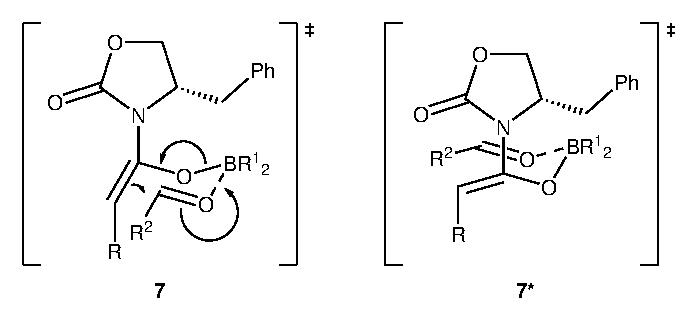
\includegraphics[width=0.68\textwidth]{2024/Abbildungen/Auxiliarchemie/4.eps}
\end{figure}
 
\enumaufgabe{\operator{Gib} jeweils \operator{an}, ob sich die Reste R und R² in axialer oder äquatorialer Position befinden. \operator{Begründe} kurz, warum die jeweils andere Position im Übergangszustand nicht auftritt.}

\solution{R: axial, R²: äquatorial (je 0,5 P.) \\
R ist axial, da die Doppelbindung (Z)-konfiguriert ist. (0,5 P.) \\
R² ist äquatorial, da beide Positionen möglich wären und äquatorial sterisch besser ist (0,5 P.). \\
insg. 2 P.}{5cm}

\enumaufgabe{\operator{Gib} das Produkt der Aldol-Reaktion in Skelettformel unter Beachtung der Stereochemie \operator{an}. }
\solution{\begin{figure}[H]
    \centering
    
\includegraphics[width=0.4\textwidth]{2024/Abbildungen/Auxiliarchemie/L_e.eps}
\end{figure}
Stereochemie 1,5 P. (jeweils 0,5 P.); alles rechts vom Carbonyl-C (nicht reaktiv) 0,5 P.; reagiertes Zentrum 2 P. \\
auch mit OH-Gruppe OK\\
Insg. 4 P.}{9.5cm}

Titan-\textsc{Lewis}-Säuren weisen mehr Koordinationsstellen auf als Bor-\textsc{Lewis}-Säuren. Bei Verwendung des Enolats \textbf{6a} wird ein anderes Stereoisomer als Produkt erhalten. 
\begin{figure}[H]
    \centering
    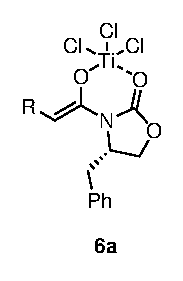
\includegraphics[width=0.18\textwidth]{2024/Abbildungen/Auxiliarchemie/5.eps}
\end{figure}
\enumaufgabe{\operator{Gib} den sechsgliedrigen Übergangszustand der Aldol-Reaktion mit dem Enolat \textbf{6a} \operator{an}. \\Hinweis: Kennzeichne gebildete und gebrochene Bindungen.}
\solution{\begin{figure}[H]
    \centering
    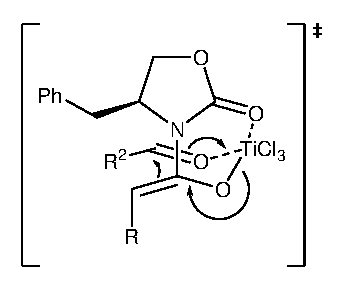
\includegraphics[width=0.4\textwidth]{2024/Abbildungen/Auxiliarchemie/L_f.eps}
\end{figure}
Sessel 0,5 P., Koordiantion von Ti 1 P., R² equatorial 0,5 P., richtige DB-Konfiguration 0,5 P. mit ax-Substituenten, 0,5 P Elektronenpfeile, 1 P Angriff von richtiger Seite\\
Insg. 4 P.}{8cm}
Mit dem Enolat \textbf{6a} sind zahlreiche weitere Reaktionen möglich, beispielsweise eine Methylierung. 
\begin{figure}[H]
    \centering
    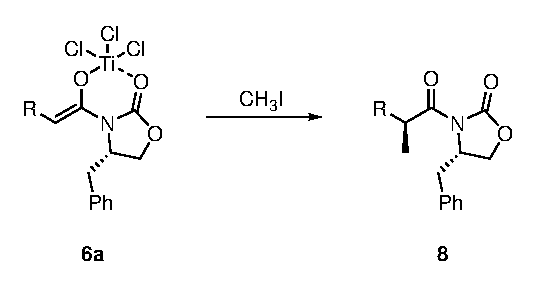
\includegraphics[width=0.55\textwidth]{2024/Abbildungen/Auxiliarchemie/6.eps}
\end{figure}

\enumaufgabe{\operator{Gib} die Konfiguration aller Stereozentren in \textbf{8} \operator{an}. Nimm dafür an, dass \textbf{R} eine Ethylgruppe ist.} 
\solution{Beide Stereozentren (S) (je 0,75 P.)}{2cm}
\enumaufgabe{\operator{Gib an}, wie viele Stereoisomere von \textbf{8} insgesamt existieren, wenn es sich bei R um eine Ethylgruppe handelt.}

\solution{4 (0,5 P.)}{1cm}

\newpage
Ein synthetisch schwerer zugängliches Enolat ist \textbf{6b}. 
\begin{figure}[H]
    \centering
    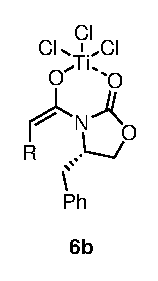
\includegraphics[width=0.125\textwidth]{2024/Abbildungen/Auxiliarchemie/7.eps}
\end{figure}
\enumaufgabe{\operator{Gib} das Produkt der Methylierung von \textbf{6b} \operator{an}.}

\solution{
\begin{figure}[H]
    \centering
    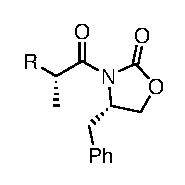
\includegraphics[width=0.26\textwidth]{2024/Abbildungen/Auxiliarchemie/L_i.eps}
\end{figure}
(1,5 P.)}{6cm}

Nach der Reaktion muss das \textsc{Evans}-Auxiliar als Hilfsstoff wieder abgespalten werden, wofür es mehrere Möglichkeiten gibt. 

\begin{figure}[H]
    \centering
    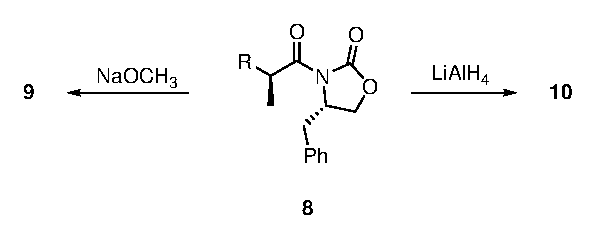
\includegraphics[width=0.58\textwidth]{2024/Abbildungen/Auxiliarchemie/8.eps}
\end{figure}
 
\enumaufgabe{\operator{Gib} die Strukturformeln von \textbf{9} und \textbf{10} \operator{an}.} 

\solution{9 \& 10:
\begin{figure}[H]
    \centering
    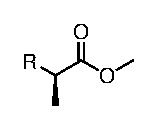
\includegraphics[width=0.2\textwidth]{2024/Abbildungen/Auxiliarchemie/L_j9.eps} \qquad \qquad
    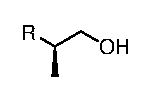
\includegraphics[width=0.2\textwidth]{2024/Abbildungen/Auxiliarchemie/L_j10.eps}
\end{figure}
(je 1 P.)\\
insg. 2 P.}{4.5cm}
\solutiontext{$\sum$ 21,5 P.}{}

\begin{comment}
    

\subsection{Ab hier würde ich alles streichen, sonst wird es zu viel
}



Enantioselektive Synthesen sind auch ohne Auxiliar möglich – mit enantiomerenreinen Katalysatoren. Im Folgenden ist eine Mannich-Reaktion mit Jörgensen-Hayashi-Katalysator \textbf{11} gezeigt. Dabei reagiert der Katalysator zunächst mit einem Aldehyd \textbf{12} zu einem Enamin \textbf{13}, welches dann an das Imin \textbf{14} addiert. Im Übergangszustand \textbf{15} sind die Stickstoffatome in räumlicher Nähe, um die entstehenden Ladungen zu stabilisieren. Nach Abspaltung des Katalysators wird das Produkt \textbf{16} erhalten. Bei TMS und PMP handelt es sich um Schutzgruppen, deren Struktur nicht relevant ist. 


\begin{figure}[H]
    \centering
    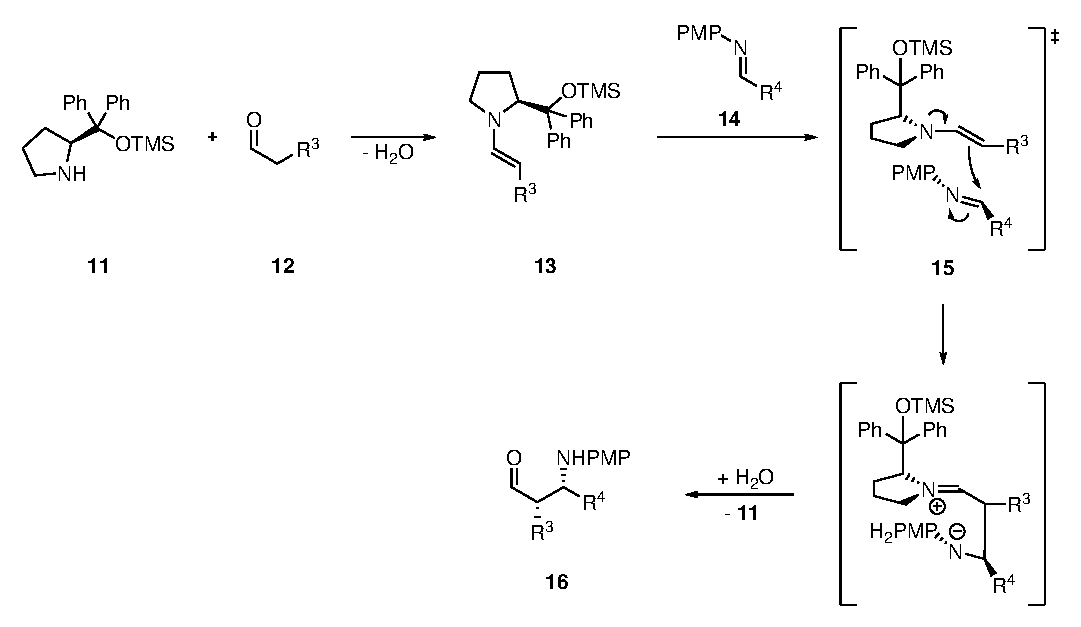
\includegraphics[width=\textwidth]{2024/Abbildungen/Auxiliarchemie/9.eps}
\end{figure}

Wird die Reaktion hingegen mit Prolin \textbf{17} als Katalysator durchgeführt, wird ein analoges Enamin \textbf{18}, aber ein anderes Produkt \textbf{19} erhalten. 

\begin{figure}[H]
    \centering
    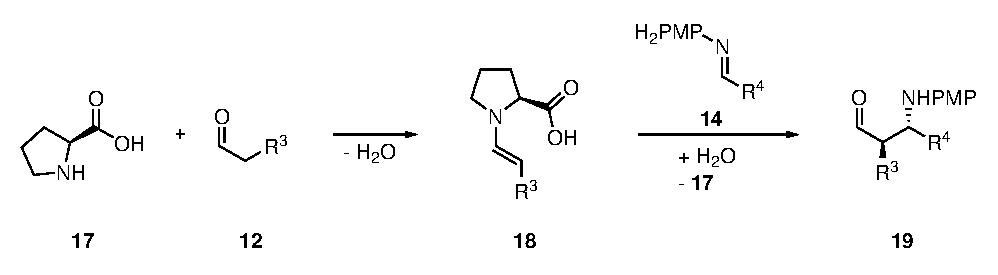
\includegraphics[width=\textwidth]{2024/Abbildungen/Auxiliarchemie/10.eps}
\end{figure}

 
\enumaufgabe{\operator{Gib} den Übergangszustand \operator{an}, der die Bildung von \textbf{19} erklärt.}

\solution{
\begin{figure}[H]
    \centering
    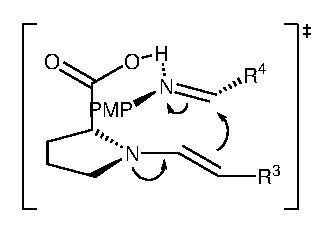
\includegraphics[width=0.3\textwidth]{2024/Abbildungen/Auxiliarchemie/L_k.eps}
\end{figure}
(4,5 P.)}{6cm}

\enumaufgabe{\operator{Gib} einen Vorteil der chiralen Katalyse gegenüber der Verwendung von Auxiliaren \operator{an}.}

\solution{Keine stöchiometrische Menge notwendig / weniger Abfall / keine zusätzlichen Schritte für Einbau und Abspaltung (1 P.)}{2,5cm}
\end{comment}
\end{document}